\documentclass[a4paper,11pt]{article}
\usepackage{tikz}
\usetikzlibrary{decorations.pathreplacing}
\usepackage{amsmath}
\usepackage{amsfonts}
\usepackage{amssymb}
\usepackage[margin=1in]{geometry}
\usepackage{graphicx}
\usepackage[utf8]{inputenc}
\usepackage[]{geometry}
\usepackage{inconsolata}
\usepackage{courier}
\usepackage{listings}
\usepackage{enumerate}
\usepackage{float}
\usepackage{answers}
\usepackage[utf8]{inputenc}
\usepackage[english]{babel}
\usepackage{commath}
\usepackage[labelfont=bf]{caption}
\usepackage{mwe}
\usepackage[longnamesfirst]{natbib}
\usepackage{algorithm}
\usepackage[noend]{algpseudocode}
\usepackage{eurosym}
\usepackage{siunitx}
\usepackage{ctable}
\usepackage{subfig}
\usepackage{dsfont}

\setlength{\parindent}{0pt}
\setlength{\parskip}{1em}

\title{Maintenance Policies for a Multi-Unit System with Adjustable Production Rates}
\author{Mark van der Broek}
\date{\today}

\begin{document}
	
	\maketitle

\section{Introduction}	
We consider a multi-unit system that consists of $n$ identical units. Each unit deteriorates according to a discrete-time Markov chain with deterioration states $X = \{0, 1, \dots, L\}$. State $0$ represents the as-good-as-new state and state $L$ the failed state. The system also allows to adjust the production rate of each unit, which has an impact on the deterioration process of the unit. The units deteriorate independently of each other, and we can perfectly observe this deterioration level for each unit at any moment in time. An graphical overview of the order of events within a time epoch is presented in Figure 1.

\begin{figure}[H]
	\centering
	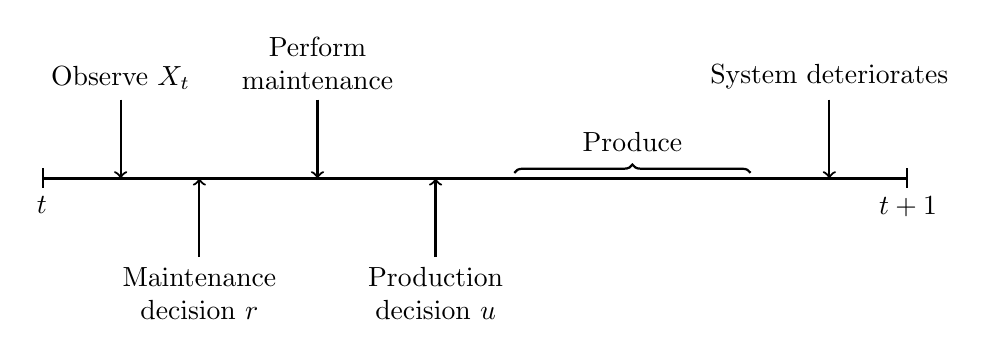
\begin{tikzpicture}
	\coordinate (t) at (0,0);
	\coordinate (X) at (1,0);
	\coordinate (R) at (2,0);
	\coordinate (M) at (3.5,0);
	\coordinate (U) at (5,0);
	\coordinate (UE) at (9,0);
	\coordinate (D) at (10,0);
	\coordinate (t+1) at (11,0);
	
	% Draw the time horizon
	\draw[thick, |-|] (t) -- (t+1);
	\draw (t) node[below=3pt] {$t$};
	\draw[thick, ->] (1,1) node[above, align=center] {Observe $X_t$} -- (X);
	\draw[thick, ->] (2,-1) node[below, align=center] {Maintenance \\ decision $r$} -- (R);
	\draw[thick, ->] (3.5, 1) node[above, align=center] {Perform \\ maintenance} -- (M);
	\draw[thick, ->] (5, -1) node[below, align=center] {Production \\ decision $u$} -- (U);
	\draw[thick, decorate, decoration={brace,raise=2pt, amplitude=3pt}] (6,0) -- (9, 0) node[sloped,midway, above=6pt] {Produce};
	\draw[thick, ->] (10, 1) node[above, align=center] {System deteriorates} -- (D);
	\draw (t+1) node[below=3pt] {$t+1$};
	\end{tikzpicture}
	\caption{Order of events for time epoch $t$.}
\end{figure}


For the analysis I will consider a system of two units, and if time permits we will relax this assumption to consider a system with more units. For the maintenance policy can perform maintenance or not with cost $c_\text{pm}$ if the unit has not failed yet and cost $c_\text{cm}$ if it has failed. The cost of preventive maintenance is assumed to be less than corrective maintenance cost ($c_\text{pm} < c_\text{cm}$). Furthermore, for any time period we do perform maintenance a fixed cost $C$ has to be incurred. Therefore, depending on the size of these three costs it could be beneficial to cluster the maintenance actions.

\section{Markov Decision Process}

The system is modelled using a Markov Decision Process (MDP) with an infinite horizon. The system consists of $n$ identical units, each with $L+1$ deterioration states. We denote the set of units as $\mathcal{I} = \{1, \dots, n\}$. For unit $i \in \mathcal{I}$ we define the state as $x_i \in X$. The whole state of all units is denoted by
$$
x = (x_1, \dots, x_n).
$$

For each unit the set of actions at each decision epoch is to decide on the production rate, and to do no maintenance (DN) or to perform maintenance (M). The action space for the maintenance decision can be defined as
$$
R = \left \{r = (r_1, \dots, r_n): r_i \in \{\text{DN}, \text{M}\}, \enskip \forall i \in \mathcal{I} \right \}.
$$
Each unit can produce at most $m+1$ different production rates, ranging from $0$ to $1$ (maximum production). The possible production rates are uniformly distributed over the interval, i.e. $u_i \in \{j / m \mid j = 0, 1, \dots, m\}$. We let $u = (u_1, \dots, u_n)$ denote the production rate of all units in the system. The total production of the system is restricted to $\pi$, i.e., $ \sum_{i=1}^{n}u_i = \pi$. In practice this is relevant, since the production rate of a system could be set by the controlling party to, for, example, comply with a contracted output rate. Adding this restriction results in the following action space for the production
$$
U = \left\{ u \mid  \sum_{i=1}^{n}u_i = \pi \right\},
$$
Note that the production action space decreases from $p^n$ elements to ${n + \pi - 1} \choose{\pi - 1} $ by restriction the total production rate to the value $\pi$.  The entire action space consisting of the maintenance and production action space is given by
$$
A = R \times U 
$$

To define the immediate rewards and transition probabilities for the system, we define a function
$$
c(x_i,r_i) = \begin{cases}
c_{\text{pm}} & \text{ if } r_i = \text{M} \text{ and } x_i \neq L, \\
c_{\text{cm}} & \text{ if } r_i = \text{M} \text{ and } x_i = L, \\
0 & \text{ elsewhere}.
\end{cases}
$$
for all states $x_i$ and maintenance actions $r_i$ of unit $i \in \mathcal{I}$.  The state and action dependent immediate cost $\bar{c}(x,r)$ for the system is given by
$$
\bar{c}(x,r) = \begin{cases}
C + \sum_{i=1}^{n}c(x_i, r_i), &\text{if } r \text{ contains a maintenance action},\\
0, &\text{otherwise}.
\end{cases}
$$
Note that if we select action $a = (u, r)$ in state $x$, then $\bar{c}(x, a) = \bar{c}(x,r)$.

\subsection{Deterioration Process}
The transition probabilities for all units are identical and independent. Each unit $i$ deteriorates according to a Poisson process with rate $\lambda(u_i)$, which depends on the current production rate of the unit. This function for a given production rate $u_i$ is given by
$$
\lambda(u_i) = g(u_i) \lambda_{\text{max}},
$$
where $\lambda_{\text{max}}$ is the rate parameter under the maximum production rate, and $g$ is some non-decreasing function. For now we assume that $g(u_i) = u_i$. For a unit $i$ the probability of having $q \geq 0$ jumps in the deterioration states for a time epoch under production rate $u_i$ is given by
$$
p(u_i,q) = \frac{\lambda(u_i)^q}{q!}e^{-\lambda(u_i)}.
$$
The transition probability of unit $k$ for going from state $i$ to $j$ with production rate $u_i$ and maintenance action DN for any time epoch is defined as
$$
P_{u_k,\text{DN}}(i,j) = \begin{cases}
p(u_k, j-i) &\text{ if } i \leq j \leq L-1, \\
0 &\text{ if } j < i, \\
1 - \sum_{l=0}^{L-1-i}p(u_k,l) & \text{ if } i \leq m-1  \text{ and } j = L, \\
1 & \text{ if } i = j = L,
\end{cases}
$$
and for maintenance action M by
$$
P_{u_k,\text{M}}(i,j) = \begin{cases}
	p(u_k, j) &\text{ if } j \leq  L-1, \\
	1 - \sum_{l=0}^{L-1}p(u_k,l) & \text{ if } j = L.
\end{cases}
$$
Note that for the maintenance action M the probability of going from state $i$ to $j$ does not depend on $i$, since we assume that the system will go to state 0 instantaneously.

The transition probability of a unit in the system is independent of the other units. Therefore, the transition probability that the system goes from state $x = (x_1, \dots, x_n)$ to state $\tilde{x} = (\tilde{x}_1, \dots, \tilde{x}_n)$ by selecting production rates $u$ and maintenance actions $m$ is given by
$$
p(x, \tilde{x} \mid u, m) = \prod_{i = 1}^nP_{u_i,m_i}(x_i, \tilde{x}_i),
$$
due to independence of the deterioration process of the units.

Let $\boldsymbol{\sigma} = (\sigma, \sigma, \dots)$ be a stationary deterministic policy. This policy induces the cost process $\{X_t, \bar{c}(X_t, d(X_t))\}$, where $d(X_t)$ is the action for state $X_t$ corresponding to policy $\boldsymbol{\sigma}$. The average cost $g$ for this problem with policy $\boldsymbol{\sigma}$ for initial value $X(0) = x$ is given by
$$
g^{\boldsymbol{\sigma}}(x) = \lim_{N \to \infty}\frac{1}{N}\left \{\mathbb{E}^{\boldsymbol{\sigma}}_x \sum_{i=0}^N\bar{c}(X_i, d(X_t)) \right\}.
$$
Our goal is to minimise to find a policy $\boldsymbol{\sigma}^*$ such that the average cost $g$ is minimised. A Successive Approximation algorithm can be used to find the minimising policy.

\section{Extensions}
A list of extensions (ordered by priority) is given below:
\begin{enumerate}
	\item Let the deterioration process of the units be modelled by a gamma process.
	\item Consider other forms for the function $g$, e.g., see what happens when this function is convex or concave.
	\item Study a system with more than two units.
	\item Add revenue instead of imposing a restriction on the total production.
	\item Add lead time for maintenance.
	\item Study dependency of deterioration process of units. For windmills one could imagine that the deterioration is partially determined by weather conditions which are identical for windmills within a wind park.
	\item Consider imperfect condition information.
\end{enumerate}


\end{document}